\documentclass[conference]{IEEEtran}
\usepackage{float}
\usepackage{graphicx}
\usepackage[pdftex,
			final,
            pdfauthor={Robin Klusman and Luc Gommans},
            pdftitle={Using imo.im in Forensic Investigations},
            pdfkeywords={imo.im, imo, forensics}]{hyperref}
\usepackage{wrapfig}
\usepackage{booktabs}
\hypersetup{
	colorlinks=true,       % false: boxed links; true: coloured links
	linkcolor=blue,        % colour of internal links
	citecolor=blue,        % colour of links to bibliography
	filecolor=magenta,     % colour of file links
	urlcolor=blue
}

%package list
\usepackage[
    backend=bibtex,
    style=numeric,
    sorting=none,
    maxcitenames=2
]{biblatex}


%\addbibresource{main.bib}
\bibliography{references.bib}


\begin{document}

\title{Using {\it imo.im} in Forensic Investigations \\\vspace{5mm} \large  \today}
\author{
\IEEEauthorblockN{Robin Klusman}
\IEEEauthorblockA{
Security and Network Engineering \\
University of Amsterdam \\
robin.klusman@os3.nl}
\and
\IEEEauthorblockN{Luc Gommans}
\IEEEauthorblockA{
Security and Network Engineering \\
University of Amsterdam \\
os3-ccf@lucgommans.nl}
}
\maketitle
\thispagestyle{plain}
\pagestyle{plain}

\begin{abstract}

    This paper presents an investigation into what forensically interesting data
    can be gathered from the imo on the Android platform. Imo is a messaging and
    voice and video calling application with over half a billion installations
    worldwide on the Android platform alone. This study investigates both what
    data is available on the local storage of a mobile device on which imo is
    used and what data can be gathered by capturing and examining network
    traffic. We find that significant amounts of data can be retrieved from the
    local storage, such as message and call data. The network traffic proved
    better secured, as we were only able to retrieve sticker data from it.

\end{abstract}

\section{Introduction}

In recent years, mobile communication tools have gained massively in
popularity. Many mobile device users nowadays use internet-based third party
messaging and calling applications over the short message service (SMS) and
regular phone calls provided by telecommunication companies.  The advantage of
these internet-based alternatives is often the more extensive features and
lower cost compared to SMS. It is therefore unsurprising that many such
applications have over hundreds of millions of downloads, making the use of
them widespread. This fact is important for forensics purposes because there
are reasonable odds that a suspect has installed and used at least one such
application, possibly to send or receive sensitive data relevant to the case.
The investigation into what data useful in a forensic investigation can be
gathered from such applications, therefore becomes very relevant.

One example of such an application is {\it imo.im}, which exists for Android,
iOS, Mac OS X and Windows \cite{imo}. It currently has over half a billion
installs on Android through the Google Play Store, which fewer than ten
messaging applications have achieved as of October 2017
\cite{wiki-gplay-popular}. This makes it a relatively widespread application on
the Android platform. Imo appears to be most popular in southern Asia and the
middle east, though there are users worldwide. In this paper we limit ourselves
to the Android version of imo due to both the prevalence of Android devices in
general, and the prevalence of imo on this platform. We expect that the
investigation of other platforms will yield similar results to the present
investigation.

\begin{figure}
	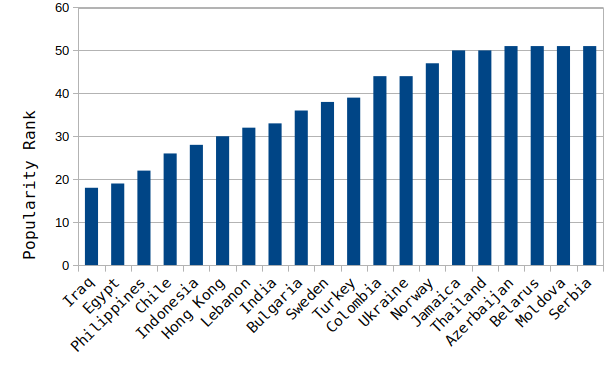
\includegraphics[width=\linewidth]{pop.png}
	\caption{Popularity ranking (lower rank means more popular) of imo per region for the top 22 regions based on data from \texttt{similarweb.com}}
	\label{fig:pop}
\end{figure}

In addition to its prevalence, imo requests permission to track its users'
location, making it even more interesting for forensic purposes. If the
application indeed tracks and stores a log of a user's location data, such data
could be valuable in court to for instance validate or invalidate a suspect's
alibi.

The remainder of this paper is structured as follows: the next section briefly
introduces the features of imo. Section \ref{sec:researchq} describes our main
research question and the defined sub-questions. In Section \ref{sec:ethics} we
discuss the ethical implications of our work. Section \ref{sec:relwork} gives
an overview of the prior work done in this area of research. In Section
\ref{sec:method} we discuss our methods and experimental setup. Section
\ref{sec:network} describes our findings from the network analysis while
Section \ref{sec:storage} describes our analysis of the mobile device's local
storage. We discuss our results in Section \ref{sec:disc} and draw conclusions
in Section \ref{sec:conc}. Finally, we present some directions for future work
in Section \ref{sec:futwork}.


\section{Overview of imo}

As stated previously, imo is a messaging and voice and video calling
application developed for Android, Mac OS X, iOS and Windows \cite{imo}. This
description focuses on the Android version of imo, as the versions for other
platforms are not investigated in this paper.

Imo requires users to log in using their phone number, and each login is
verified through an SMS code sent to that number. There is no difference
between logging into an existing account (i.e. phone number known and
previously used for imo) and creating a new account (i.e. phone number not
previously used for imo), as imo uses the same procedure for both. There are no
other types of logins possible, e.g. there is no option to register using a
username and password.

Note that multiple devices can use a single number at the same time. The app
does not show this to the user and crashes regularly in this set-up.

Contacts in imo are added through your Android phone book. You can send those
contacts text messages, or place (video) calls. You can also share a `story',
which is a graphical message shared with all your contacts. It can consist of a
picture, short video, drawing, etc. Contacts can view your stories and send a
response. These responses appear in the chat history of that contact as a
reply, referencing your story.

When chatting, the message you are typing is immediately visible to the other
party, before even sending it. This (default-enabled) feature is called `Real
time chat'. Sending a message makes it final: it cannot be edited afterwards,
and one can only delete it locally.

Imo also supports group chats and group calls. Compared to regular chats, we
did not find these to have any special features.

Finally, imo supports what are called `stickers': large, animated emoticons.
These are placed in a chat as a message by themselves.


\section{Research Questions}\label{sec:researchq}

Our main research question is:
{\it What information can be gathered from the `imo' messenger app for Android?}

\vspace{0.1cm}

\noindent{} This main research question divides in four sub-questions:

\begin{enumerate}
    \item What data is identifiably sent over the network?
    \item What data is available locally?
    \item What location data is available locally or identifiably sent over the
        network?
    \item Do any cached files or images exist locally?
\end{enumerate}


\section{Ethical Considerations}\label{sec:ethics}

For this paper we will use a test environment to examine the data that can be
extracted from the imo Android app. We will not be using any real user data and
use only designated test devices to make sure we do not invade or compromise the
privacy of any real imo users.


\section{Related Work}\label{sec:relwork}

No prior work has been done on the imo messaging app for any platform, the only
mention of imo in academic literature is in the paper by \citeauthor{zhu},
which does a more general review of several group messaging applications and
does not conduct an analysis of what data can be acquired for use in a criminal
investigation \cite{zhu}.

Fortunately, academic research does exist on the forensic investigation of
other messaging applications. \citeauthor{mahajan2013forensic} conduct a
forensic analysis of the Android messaging applications Viber and WhatsApp
\cite{mahajan2013forensic}. The aim of their paper is to find whether the data
of those applications, such as sent and received messages and images, are
stored locally in a way that they can be extracted from the device.
\citeauthor{mahajan2013forensic} managed to find and extract several artifacts
relevant to a forensic investigation, such as sent and received messages and
contact phone numbers.

\citeauthor{walnycky2015network} conduct an extensive investigation of 20
popular Android messaging applications \cite{walnycky2015network}. In their
paper they investigate what data is can be retrieved by investigating the
mobile device's local storage, the applications' server storage and network
traffic analysis in a forensic investigation for each application. For the
purpose of cross-referencing the results, network traffic is analysed using
three different tools: Wireshark, NetworkMiner and NetWitness Investigator.
Server-stored data was investigated by recovering links to the applications'
servers from the network traffic analysis. Locally stored data was acquired and
investigated using Micro-systemation's {\it XRY} and verified by also using
{\it Helium backup} in combination with {\it Android backup extractor} and an
SQLite database browser.  In their paper, \citeauthor{walnycky2015network}
state that 4 of the applications leaked no data when subjected to their
investigative methods.  However, their study did find that 16 applications do
leak data either through network communication or local/server storage.

A forensic investigation of WhatsApp is also conducted by
\citeauthor{anglano2014forensic} \cite{anglano2014forensic}, who uses a virtual
Android environment created with {\it YouWave} to investigate what data can be
acquired from WhatsApp through a device's local storage. Their study shows that
it is very feasible to acquire WhatsApp data from local storage, since data
such as sent and received messages and contact information is stored
unencrypted on the local storage.


\vspace{0.2cm}
\section{Methods}\label{sec:method}

To investigate what forensically interesting data can be obtained through imo,
we first focus on analysing network traffic. For this analysis, we run a
tcpdump locally on the phone, writing the data in pcap format to a file. We
then download the data from the phone and inspect it using Wireshark
afterwards. The results of this are discussed in Section \ref{sec:network}.

The investigation of the local storage is done by first imaging the local data
partition of the device using \textit{dd} from the ADB shell. We then mount
this image read only on our Linux system. Analysis of the image was done
manually, the results of this investigation are discussed in Section
\ref{sec:storage}.


\subsection{Experimental Setup}\label{sec:setup}

For our analysis of imo we used two Android phones, a Sony Xperia Z (C6603) and
an Alcatel Pixi 4, both of which run Android version 6.0.1. The imo application
has versionCode 0x709 and the versionName is `9.8.000000009731', according to
the \texttt{AndroidManifest.xml} file inside the APK. The SHA-256 hash value of
the APK file is \texttt{61972382 e73a4614 0cae38a0 3eae8b63 9f6e42aa 9d47368d
f207a08b a6f097ae}.


\vspace{0.3cm}
\section{Network Communication Analysis}\label{sec:network}

Upon analysing the pcap file in Wireshark, we found that the regular network
communication (e.g. chats) use TCP ports 443, 5223 and 5228. We have not been
able to identify why the app sometimes uses one port over the other. In the
APK, we find references to those three ports together, so we are confident that
there are no other TCP ports in use.  Searching online for those ports, we find
that these ports overlap with WhatsApp, C2DM (now-defunct server-push platform
provided by Google, using port 5228) and Apple's push implementation (APNS,
using port 5223). Most likely, imo uses those ports because they are commonly
used by mobile devices for core operating system features (server push) or
other popular applications. Network administrators are unlikely to block those
ports.

The downloading of stickers is done over plain HTTP. Anyone observing the
network traffic can therefore see which emoticons are used by a device. It is
not visible, however, which chat a sticker was used in. Stickers are also
cached, so they will not be downloaded twice, also between for example reboots.
How long they will be cached exactly, is unknown. In our tests, the client
never checked for new versions (we expected to see `if-modified-since' or
`if-none-match' HTTP headers).

UDP is used for voice and video calls, using various ports. The choice of UDP
port seems random for the server, though we have also twice observed the server
to use UDP port 443 which seems too specific to be a coincidence, particularly
because it happened twice. The lowest port observed, other than 443, is 29 879.
Possibly a port is picked above a certain number to avoid conflicts with
existing services.

The Android client also appears to choose ports at random, though the lowest we
have observed was 33 419. We theorise that a random port is chosen above 32 000
to avoid using another service's port.

The clients involved in a call will try to reach each other directly for voice
and video calls. The communication goes through imo's servers by default, but
the app keeps trying to communicate peer to peer throughout the whole session
(it sends a packet twice per second). If this succeeds, it will switch to peer
to peer communication. After switching, calls continue to work even when the
connection to imo's servers is disrupted, e.g. when the clients are in one LAN
and the internet connection is turned off.


\subsection{Communication Format}

Any stickers used in chats are downloaded over TCP port 80, using HTTP/1.1. A
sticker is a ZIP archive with images in PNG format, one per frame of the
animation. The filenames are sequential numbers: \texttt{1.png},
\texttt{2.png}, etc. When the user is picking a sticker, the previews are
downloaded as a single image over HTTP (rather than the full animation in a ZIP
archive).

When the app chooses to use port 443 for any part of its communication, the
connection is secured using TLSv1.2. The client offers 20 cipher suites, among
which obsolete ciphers such as \texttt{TLS\_RSA\_WITH\_RC4\_128\_SHA} and
\texttt{TLS\_RSA\_WITH\_AES\_128\_CBC\_SHA}, though this is probably dependent
on the operating system. In our case, the server picked
\texttt{TLS\_RSA\_WITH\_AES\_128\_GCM\_SHA256}, which is labelled by Mozilla as
a cipher suite of intermediate strength\cite{moz-tls}.

When the app chooses to use one of the two alternative TCP ports (5223 or
5228), the connection is encoded using an unknown method. The data is binary
and could be compressed, encrypted or both. When sending multiple kilobytes of
repeating characters, the observed traffic is much smaller, leading us to
believe the data is compressed. Since decoding as TLS fails in Wireshark, and
since no readable strings are visible at all, we believe that the traffic is
not any version of TLS.

The size of these packets is always divisible by 16 bytes and in the source
code we find a static 128-bits AES key and references to AES-CBC with PKCS5
padding. We also find code to decrypt data using an IV of all zeroes. When
attempting to decrypt the traffic using this static key and the zeroed IV, or
when we interpret the first 128 bits of a stream as the IV, we only find
unrecognisable binary data. Whether the data is truly encrypted is unknown.
Since compression will also result in high entropy estimations, we cannot use
this method to determine whether it is encrypted.

We have not been able to identify the protocol used for UDP traffic. For the
traffic which is sent over port 443, we tried to decode it using Wireshark as
DTLS and QUIC traffic, but neither was successful. The traffic also does not
contain any strings, such as the common name or issuer name from a certificate,
which should have been visible for normal TLS or QUIC traffic. Packets over UDP
are of irregular lengths, often as short as 10 bytes and often not divisible by
even numbers. We find a few predictable bytes, such as an incremental number
which could be used as a counter for encryption, but not enough to draw any
conclusions about the encryption used (if any).


\subsection{Recognisability}

On TCP port 443, where TLSv1.2 is used, a certificate with `commonName'
\texttt{*.imo.im} is used, issued by Thawte. The organisation name is
`PageBites Inc.'. The certificate is valid for a period of about 20 days.

When the application uses TCP ports 5223 or 5228, the data appears completely
random. We could not identify a recognizable sequence. One might guess that
this is imo traffic by ruling out other applications which use this port, or by
observing the traffic switching between those three ports. Once it decides to
connect over TCP port 443, it can be recognized as described before.

In the UDP traffic we did observe some patterns, but we did not see a clear
marker which could readily be used for identification.


\section{Local Storage Analysis}\label{sec:storage}

After mounting the mobile device disk image, we found that most of the data
used by imo is stored in the application's own data directory:
\texttt{/sdcard/Android/data/com.imo.android.imoim}. Imo also stores some data
in \texttt{/sdcard/DCIM/imo} and \texttt{/sdcard/IMO} however, only video and
picture data used in conversations or stories are stored here.

In the data directory, we can find all our messages and contacts in the SQLite3
file \texttt{databases/imofriends.db}. For all contacts, both their name and a
numeric \texttt{buid} is stored. Group chats are also stored with their
name/identifier but use a non-numeric \texttt{buid}.

The table `messages' contains all messages, including whether a message was
delivered to the recipient's device and whether a message was read (the columns
\texttt{message\_state} and \texttt{message\_read} are set to `1' when
delivered and read, respectively).

The table `call\_timestamps' contains a convenient log of all calls placed
through the imo application. Only the start time is noted, together with the
contact which was called, not the end time or duration. This timestamp is in
Unix format, in nanoseconds, in the UTC timezone. Missed calls are placed in
the `messages' table, as a chat message to the respective user.

The table `friends' contains your contacts. These are all the people you can
message and call. In contrast, the tables `imo\_phonebook', `phone\_numbers',
and `phonebook\_entries' contain all contacts of whom you have a number; these
contacts are the ones also in your Android contact list. If the contact is not
on imo, they will not appear in `phone\_numbers'. It appears that you are only
able to see stories of the users of whom you have the number.

Outside of this database, other files also contain usage information. The JSON
file \texttt{files/brefs.json} contains a field named
\texttt{LAST\_APP\_OPEN\_TS}, which contains a timestamp of when the app was
last opened.

We find no trace of messages communicated through the `real time chat' feature,
neither on the sender's nor the receiver's side.


\subsection{Logged-in User Data}

When signing up or logging in, the phone number entered is stored in
\texttt{files/VerificationPrefs.json}, even before the confirmation code sent
through SMS is entered to confirm the number.

After confirming the number, it is also stored in \texttt{files/bprefs.json}.
The JSON file contains a field named \texttt{GET\_MY\_PROFILE}, which is
another JSON string containing a field named \texttt{phone}. This file also
contains the fields \texttt{SIGNUP\_DATE} and \texttt{SIGNUP\_TIME}, which
contain the first time someone logged in with this phone number and the last
time you logged in on this device with this number, respectively.


\subsection{Removed Data}

When you delete a message from a chat in imo, the application deletes it from
the local database's `messages' table. Similarly, when you delete one of your
stories, it is deleted from the `stories' table. However, in the binary data,
we can still find the original message. By parsing the SQLite format, one might
be able to find other fields belonging to the message such as the corresponding
timestamp.

When removing a story, references to the story are not deleted. For example
when one replies to a story, an entry is created in the `messages' table which
refers to it by its object identifier. These rows are not deleted upon deletion
of the original story. When attempting to view the story in the application via
this reference, it shows the story as having been deleted.

When removing one's account on imo, most of the local database tables are
cleared. The `call\_timestamps' table is, however, not cleared and still
contains all previous calls made on this device. Other tables, such as
`messages' and `friends', are cleared. Like with deleted messages, however, the
original data can still be found in the binary data of the SQLite file.

Finally, when we remove a contact from the Android contact list, this number is
preserved in the `phonebook\_entries' and `imo\_phonebook' tables of
\texttt{imofriends.db}.


\section{Discussion}\label{sec:disc}

Gathering data from the local storage of the imo Android application in a
forensic investigation proves very feasible, as imo does not encrypt or even
obfuscate any of this data. Additionally, much---if not all---of the data is
indeed stored locally. Imo did not opt to instead only store privacy-sensitive
data on a well-protected server and wiping it from the mobile device's local
storage.

Deletion of data is also not properly implemented. Upon deleting a contact from
your Android contact list, a copy of the name and number will remain in two
places in the local imo database. Upon deleting a message, the entry in the
database is deleted but it is still present in the binary data until it is
overwritten. This same issue applies when an entire account is deleted: data is
still available in the binary. In addition, at least one database table, the
call history table, does not have its entries removed at all. We would expect
an application that deals with private data, such as private chats, to
re-create, if not securely wipe the entire database upon account deletion to
prevent data leakage in this way.

However, the lack of data confidentiality is not wholly unexpected, as imo does
not claim to be a privacy-focused application. Normally, other apps on the
device should not be able to access imo's data directory, making data stored
here reasonably secure. Still, simple measures could have been taken to harden
the application against such situations where access to the device's local
storage is attained by an untrusted party.

Additionally, the ease with which imo's local data was accessible makes it
relatively simple for a user to alter (i.e. forge) their own data. One could
make it appear as if someone else was logged into the device, or manually
insert messages into the chat history.

Some data that we deem to be relevant in a forensic investigation could,
however, not be acquired. We were not able to retrieve unsent messages from the
local storage or network analysis (while they were communicated through the
`real time chat' feature), so imo could be used to secretly communicate through
these drafts. We were also unable to find any location data in the locally
stored data or through network analysis. It therefore remains unclear whether
or not imo gathers this data at all, but the fact imo requests location
permissions suggests that such data may indeed be gathered. The video and voice
data going through imo also remained unattainable, as such data is not stored
locally and the network traffic is sent in an unknown, possibly encrypted
format.

One should also be aware that, in imo, the same phone number can be used on
multiple devices concurrently, such as two Android phones. That an account with
a particular phone number sent a certain message, reveals little about which
device was used.

Finally, the fact that imo attempts to connect between devices directly for
voice and video calls, might reveal the IP address of the other party. Even if
the connection is unsuccessful, one can see which IP address it attempts to
reach. This might reveal which device is used, or where a user is located.


\section{Conclusion}\label{sec:conc}

As shown in this paper, significant amounts of data can be gathered from the
imo Android application, mostly from a mobile device's local storage. This data
includes sent and received messages, images and videos used in chats, which
calls were made and when, and what contacts are in this user's (imo) contact
list. Monitoring a device's network traffic yielded few results of
significance, as the data sent and received by imo is not in plain text. The
only plain text data which travels over the network, is data related to
stickers. We were unable to find any location data stored or sent by imo, and
it remains unclear what location data is collected, if any.


\section{Future Work}\label{sec:futwork}

In this paper we have left the investigation of imo on platforms other than
Android unexplored. Even though imo is most heavily used on Android,
investigating the imo versions for other platforms could still prove valuable.

We were unable to find what protocol the app uses for its communication (only
stickers were plain HTTP) when it does not use TCP port 80 or 443. We expect
that the chat communication is encrypted, but the voice and video calls over
UDP seem more likely to only be compressed and therefore susceptible to passive
intercepts. There are some predictable bytes and packets, such as an
incrementing number in what we believe to be data packets. Another incrementing
number is sent in separate, smaller packets which are sent roughly every two
seconds. The other party echoes the number in this packet. Further
investigation into the UDP traffic could both give more insight into what data
is being sent as well as helping recognize imo in intercepted traffic.

Finally, it might be possible to more precisely identify who sent a certain
message, by identifying the device it was sent from. Currently, we were only
able to identify from which phone number or imo contact a message was received.
Since one can log into the same account (i.e. use the same phone number) on
multiple devices concurrently, one cannot discern between multiple devices
using the same number. Identifying from which device a message was sent,
possibly by looking at the IP addresses that are visible in the UDP traffic,
would be valuable.


\printbibliography

\end{document}

